\documentclass{article}
\usepackage{amssymb,amsmath}
\usepackage[mathletters]{ucs}
\usepackage[utf8x]{inputenc}
\usepackage{url}
\usepackage{graphicx}
% We will generate all images so they have a width \maxwidth. This means
% that they will get their normal width if they fit onto the page, but
% are scaled down if they would overflow the margins.
\makeatletter
\def\maxwidth{\ifdim\Gin@nat@width>\linewidth\linewidth
\else\Gin@nat@width\fi}
\makeatother
\let\Oldincludegraphics\includegraphics
\renewcommand{\includegraphics}[1]{\Oldincludegraphics[width=\maxwidth]{#1}}
\usepackage[breaklinks=true,unicode=true,pdfborder={0 0 0}]{hyperref}
\setlength{\parindent}{0pt}
\setlength{\parskip}{6pt plus 2pt minus 1pt}
\usepackage{listings}
\usepackage[top=2cm,bottom=2cm,left=2cm,right=2cm,a4paper]{geometry}
\usepackage[frenchb]{babel}
\usepackage{graphicx}
\usepackage{color}
\definecolor{vert}{rgb}{0,0.5,0}
\definecolor{bleu}{rgb}{0,0,0.5}
\lstset{language=Python,basicstyle=\ttfamily\footnotesize,commentstyle=\color{vert},keywordstyle=\color{bleu}}

\title{Formation scribe}
\author{Nicolas Poulain - Dafor 2012}

\begin{document}
\maketitle

\tableofcontents

\section{Les modules EOLE}

Extrait de
\href{http://eole.orion.education.fr/index.php/home}{http}\href{http://eole.orion.education.fr/index.php/home}{://}\href{http://eole.orion.education.fr/index.php/home}{eole}\href{http://eole.orion.education.fr/index.php/home}{.}\href{http://eole.orion.education.fr/index.php/home}{orion}\href{http://eole.orion.education.fr/index.php/home}{.}\href{http://eole.orion.education.fr/index.php/home}{education}\href{http://eole.orion.education.fr/index.php/home}{.}\href{http://eole.orion.education.fr/index.php/home}{fr}\href{http://eole.orion.education.fr/index.php/home}{/}\href{http://eole.orion.education.fr/index.php/home}{index}\href{http://eole.orion.education.fr/index.php/home}{.}\href{http://eole.orion.education.fr/index.php/home}{php}\href{http://eole.orion.education.fr/index.php/home}{/}\href{http://eole.orion.education.fr/index.php/home}{home}

\begin{figure}[htbp]
\centering

\includegraphics{scribe_html_2ce1ff75.png}
\caption{Logo EOLE}
\end{figure}

Eole est un projet collaboratif basée sur la philosophie du logiciel
libre. La mutualisation des compétences et des moyens permet de réaliser
des solutions économiques, fiables et performantes.

Chaque module constitue une distribution GNU/LINUX spécifique qui permet
d'installer facilement un serveur dédié. Les services offerts sont
pré-configurés, l'ensemble est cohérent. Vous devez télécharger sur ce
site l'image ISO qui vous permettra de graver un DVD ou un CD
d'installation. Ce DVD/CD est multi module, le choix du module à
installer est proposé au démarage (boot).

Les modules sont disponibles en deux versions

EoleNg 2.2 - Disponible depuis le 16 Janvier 2009. - basée sur la
version 8.04 Ubuntu - Arrêt du support mises à jour : Juin 2013

EoleNg 2.3 - Disponible depuis le 8 Juin 2011. - basée sur la version
10.04 Ubuntu - Arrêt du support mises à jour : Juin 2015

\subsection{Scribe : Un serveur pédagogique complet.}

Scribe est un contrôleur de domaine dotée de fonctions évoluées. Il
optimise la gestion de votre parc de stations clientes. Il dispose d'un
annuaire qui référence, élèves, parents, personnels enseignant et
administratifs, il propose un service de messagerie et héberge vos
applications web au sein d'un portail Web 2.0.

Scribe est un contrôleur de domaine.

\begin{itemize}
\item
  gestion des connexions réseau des utilisateurs ;
\item
  partage de fichiers et de répertoires ;
\item
  support des ACL ;
\item
  partage d'imprimantes ;
\item
  gestion des comptes utilisateurs et des accès ;
\item
  exécution d'applications utilisateurs ;
\end{itemize}
Scribe est un système de messagerie articulé autour d'un annuaire
performant.

\begin{itemize}
\item
  l'annuaire est initialisé à partir d'importation de comptes (SCONET,
  BE1D, AAF, CSV,\ldots{}) ;
\item
  l'annuaire peut servir de base d'authentification pour d'autres
  services réseaux ;
\item
  la messagerie gère deux domaines distincts (l'Internet et l'intranet
  académique) ;
\item
  utilisation au choix d'une interface web multilingue ou d'un client de
  messagerie standards.
\item
  un service de listes de diffusion ;
\item
  une sécurité anti­spam, un anti­virus, une gestion de quotas (taille
  des boites aux lettres)
\end{itemize}
Scribe offre des services web
=\textgreater{}\href{http://eole.orion.education.fr/projects/envole/wiki/Descriptif}{}\href{http://eole.orion.education.fr/projects/envole/wiki/Descriptif}{Envole}\href{http://eole.orion.education.fr/projects/envole/wiki/Descriptif}{2.0}

\begin{itemize}
\item
  un serveur web;
\item
  un portail web;
\item
  des applications pré-installés
\end{itemize}
Scribe est un serveur d'authenfication unqiue (SSO)

\begin{itemize}
\item
  Eole SSO Utilise l'annuaire LDAP
\item
  Les standards C.A.S 2 et OpenID sont supportés
\item
  La féération d'identité est possible via le protocole SAML.
\end{itemize}
Scribe dispose d'une gestion avancée des utilisateurs et des postes
clients

\begin{itemize}
\item
  Distribution de devoir
\item
  Controle d'acces à Internet et au services réseaux
\item
  appliquer des restrictions ou pré­configurer des applications, en
  fonction du login de l'utilisateur ou de ses groupes et du nom de la
  machine sur laquelle il se connecte ;
\item
  effectuer des actions distantes sur les stations (fermer la session,
  éteindre ou redémarrer un ou plusieurs postes) ;
\item
  surveiller la détection de virus par le serveur ;
\end{itemize}
\subsection{Schéma d'un réseau d'établissement}

Sur l'académie de Paris, les réseaux d'établissement sont organisés par
la DSI, service informatique du Rectorat qui assure en plus
l'administration et la maintenance des serveurs Amon, Scribe et Horus.
Voir figure \ref{2149feac}.

\begin{figure}[htbp]
\centering
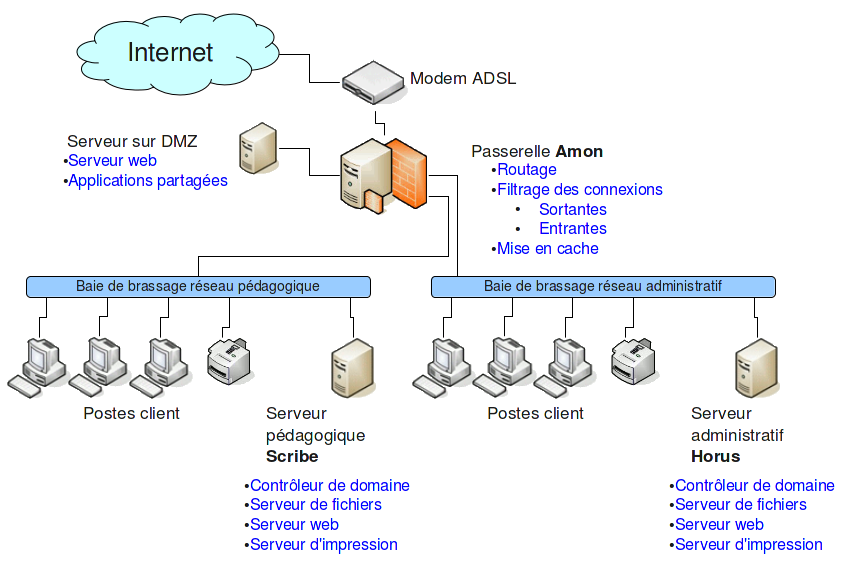
\includegraphics{scribe_html_2149feac.png}
\caption{\label{2149feac}}
\end{figure}

Les établissements assurent par eux-même les tâches de gestion courante
du réseau et des machines avec les droits qui leur sont laissé en
utilisant au travers des interfcaes de gestion de ces serveurs.

\subsection{Déroulement de la formation}

Durant cette formation, nous allons simuler un réseau d'établissement
grâce à des machines virtuelles. Cela nous permettra de contrôle
complètement tous les éléments, d'effectuer tous les tests sans risque
pour les machines réelles et le réseau qui nous entourent.

Sur la figure suivante, on simule plusieurs machines sur une seule
appelée machine hôte. Un poste windows virtuel est un ordinateur virtuel
sur leque a été installé un système d'exploitation comme on le fait sur
une machine réelle.

\begin{figure}[htbp]
\centering
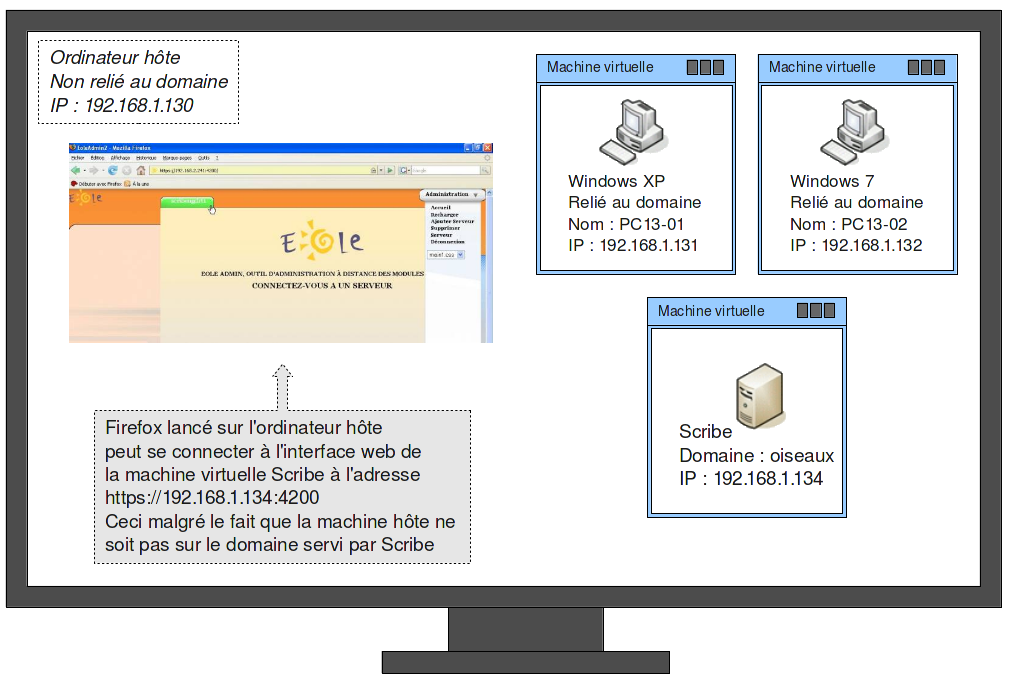
\includegraphics{scribe_html_413f4ff1.png}
\caption{\label{413f4ff1}}
\end{figure}

La situation décrite sur la figure \ref{413f4ff1} est équivalente à
celle de la figure \ref{78733841}.

\begin{figure}[htbp]
\centering
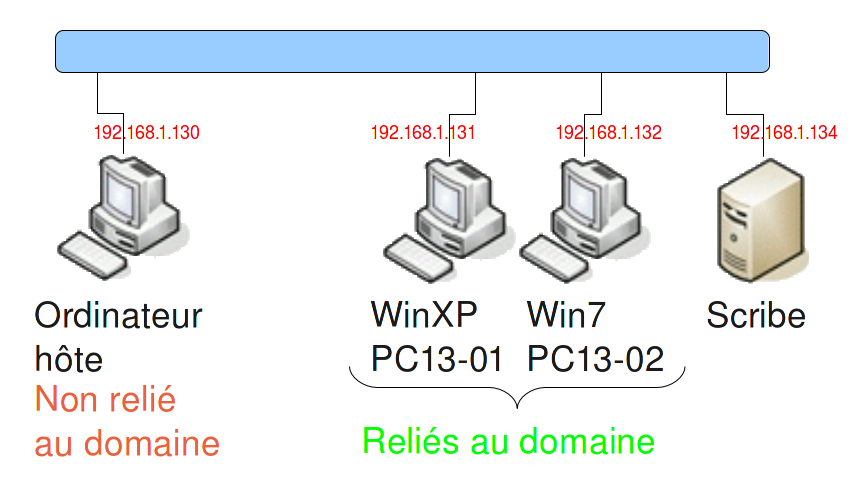
\includegraphics{scribe_html_78733841.png}
\caption{\label{78733841}}
\end{figure}

Notre travail maintenant est de créer la machine virtuelle qui va
accueillir le sytème d'exploitation Linux sur lequel fonctionne.

Après avoir demandé la création d'une nouvelle machine dans VirtualBox,
puis donné un nom (disons scribe) et choisi le type de système
d'exploitaion (ici Linux-Ubuntu), passez toutes les étapes en acceptant
les choix par défaut (sauf pour la mémoire vive que nous passerons de
512Mo à 256Mo).

Une fois ces opérations terminées,

\begin{itemize}
\item
  cocher la case \textless{}\textgreater{} dans l'onglet «Processeur» de
  la section \textless{}\textgreater{} de votre machine virtuelle.
\item
  choisir le mode d'accès par pont pour la carte réseau 1. Elle prendra
  ainsi une adresse sur le réseau sur lequel se trouve la machine hôte.
\item
  L'image iso du dvd eole, téléchargée sur le site Eole
  \url{http://eoleng.ac-dijon.fr/pub/iso/} doit être monté comme un
  cd(ou dvd) virtuel, pour cela cliquez sur l'icône cd-rom dans l'onglet
  \textless{}\textgreater{}, comme sur l'image ci-dessous puis naviguez
  dans l'arborescence pour indiquer le fichier .iso.
\end{itemize}
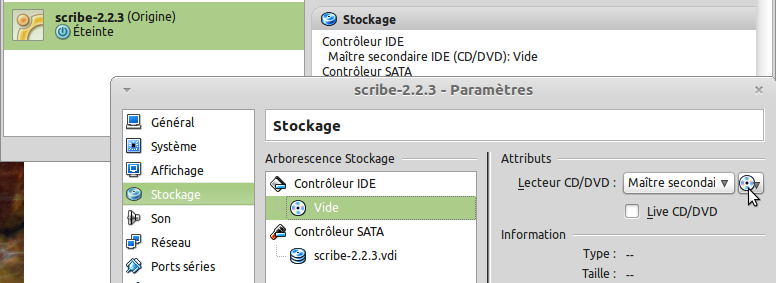
\includegraphics{scribe_html_m69a9bc5b.png}\\ On peut alors mettre en
marche la machine virtuelle.

\end{document}
